\documentclass[conference]{IEEEtran}

\usepackage{amssymb,amsmath,graphicx,float,array,theorem}
\usepackage[noadjust]{cite}
\usepackage[latin1]{inputenc}
\usepackage[dvips,ps2pdf]{hyperref}

\newcommand\real{\mathbb{R}}
\newcommand{\req}[1]{(\ref{#1})}
\newcommand{\fimex}{\hfill $\Box$}
\DeclareMathOperator{\atan}{atan2}

%\theorembodyfont{\mdseries}
\newcounter{examplecounter}
\newtheorem{ex}{Example\refstepcounter{examplecounter}}

\begin{document}

\title{Point Stabilization of Mobile Robots with Nonlinear Model Predictive Control}

\author{\authorblockN{Felipe K\"{u}hne, Walter Fetter Lages and Jo\~{a}o Manoel Gomes da Silva Jr.}
\authorblockA{Universidade Federal do Rio Grande do Sul \\
Department of Electrical Engineering \\
Av. Oswaldo Aranha, 103 \\
Porto Alegre, RS 90035-190 Brazil \\
Email: {\tt \{kuhne,fetter,jmgomes\}@eletro.ufrgs.br}}}

\maketitle

\begin{abstract}
This paper presents an optimal control scheme for a wheeled mobile robot (WMR) with nonholonomic constraints. Due to Brockett's conditions, it is well known that a smooth, static state feedback control law can not be used to stabilize a nonholonomic system at a given posture. Usual approaches consider the use of non-smooth or time-varying control laws. However, these approaches commonly present some drawbacks. Furthermore, in realistic implementations it is difficult to obtain good performance, due to the constraints on system's variables that naturally arise. By using model predictive control (MPC), a control law that respects the Brockett's conditions is implicitly obtained. One of the main advantages of MPC is the ability to handle constraints (due to state or input limitations) in a straightforward way. The point stabilization problem for a nonholonomic WMR is solved and some simulation results are shown. Also, considerations regarding the computational effort of the MPC are developed with the purpose of speculating the viability of the proposed technique in a real implementation.
\end{abstract}


%%%%%%%%%%%%%%%%%%%%%%%%%%%%%%%%%%%%%%%
\section{Introduction}\label{sec:intro}

The field of mobile robot control has been the focus of active research in the past decades. In despite of the apparent simplicity of the kinematic model of a wheeled mobile robot (WMR), the design of stabilizing control laws for those systems can be considered a challenge due to the existence of nonholonomic (non-integrable) constraints. Due to Brockett's conditions~\cite{brockett82}, a smooth, time-invariant, static state feedback control law cannot be used to stabilize a nonholonomic system at a given posture. To overcome these limitations most works use non-smooth and time-varying control laws~(see \cite{bloch89,samson91,canudas92,yamamoto94,murray97} and the references therein). Recent works dealing with robust and adaptive control of WMRs can be found in \cite{oya03,dixon04}.

In realistic implementations, traditional techniques for the control of nonholonomic mechanical systems, such as non-smooth and time-varying control laws, often do not present good results, due to the constraints on inputs or states that naturally arise. In general, the resulting closed-loop trajectory presents unnecessary oscilatory motions. Furthermore, tuning parameters are difficult to choose since these control laws are not intuitively obtained.

In this paper we show that, by using model predictive control (MPC), all these disadvantages can be overcome: the tuning parameters are easy to deal with; a cost function is minimized, which makes the control law optimal according to the optimization criterions; constraints on state and control inputs can be considered in a straightforward way during the computation of the control law. For a WMR the latter is an important feature, since the position of the robot can be restricted to belong to a safe region of operation. By considering input constraints, control actions that respect actuators' limits can be generated. Furthermore, a control law that respects Brockett's conditions is implicitly obtained.

MPC is an optimal control strategy that uses the model of the system to obtain an optimal control sequence by minimizing a cost function. At each sampling interval, the model is used to predict the behavior of the system over a prediction horizon. Based on these predictions, a cost function is minimized with respect to the future sequence of inputs, thus requiring the solution of a constrained optimization problem for each sampling interval. Although prediction and optimization are performed over a future horizon, only the values of the inputs for the current sampling interval are used and the same procedure is repeated at the next sampling time. This mechanism is known as {\it moving} or {\it receding horizon} strategy, in reference to the way in which the time window shifts forward from one sampling time to the next one.

For complex, constrained, multivariable control problems, MPC has been successfully applied in the process industries. It is used in many cases, where plants being controlled are sufficiently {\em slow} to allow its implementation. However, for systems with fast and nonlinear dynamics, which is the case of mobile robots, the implementation of predictive controllers remains fundamentally limited in applicability, due to the large amount of {\em on-line} computation required~\cite{cannon00}. However, with the development of increasingly faster processors and efficient numerical algorithms, the use of MPC in such demanding applications becomes possible. Although MPC is not a new control method, works dealing with MPC of WMRs are recent and sparse~\cite{ollero91,ortega96,yang98,rico99,essen01}.

Thus, in this paper a nonlinear MPC (NMPC) scheme is developed to the problem of point stabilization for a nonholonomic WMR. In order to improve the performance of the closed-loop trajectories, a transformation in polar coordinates is introduced in the cost function to be minimized. Also, computational effort analyses are therefore carried out to study the viability of the application of these algorithms in a real implementation.

%This paper is organized as follows: in the next section the kinematic model of the WMR and some important model properties are shown. The MPC algorithm is depicted in section~\ref{sec:mpc}. Simulation results in {\sc Matlab} are shown in section~\ref{sec:simulations} and section~\ref{sec:conclusions} the conclusions are pointed out.


\section{Kinematic Model of the WMR}
\label{sec:model}

A mobile robot made up of a rigid body and non deforming wheels is considered (see Fig.~\ref{fig:robot}). It is assumed that the vehicle moves on a plane without slipping, i.e., there is a pure rolling contact between the wheels and the ground. The kinematic model of the WMR then is given by~\cite{Campion:TRA-12-1}:

\begin{equation}\label{eqn:model}
	\left\{
		\begin{aligned}
			\dot x	  &= v\cos\theta\\
			\dot y	  &= v\sin\theta \\
			\dot \theta &= w
		\end{aligned}
	\right.
\end{equation}

\noindent or, in a more compact form as
\begin{equation}\label{eqn:modelshort}
	\dot{\bf x} = f({\bf x},{\bf u}),
\end{equation}
where ${\bf x}=[x~~y~~\theta]^T$ describes the configuration (position and orientation) of the center of the axis of the wheels, $C$, with respect to a global inertial frame $\{O,X,Y\}$. ${\bf u}=[v~~w]^T$ is the control input, where $v$ and $w$ are the linear and the angular velocities, respectively.
\begin{figure}[htbp]
	\centering
	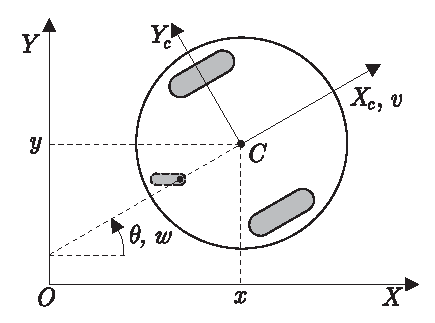
\includegraphics[width=0.67\linewidth]{Figures/robot.eps}
	\caption{Coordinate system of the WMR.}
	\label{fig:robot}
\end{figure}

For the sake of simplicity, we assume in this work that the states of the plant are always available for measurement and that there are no plant/model mismatch.

Since the MPC scheme used here is computed in discrete-time, it is necessary to discretize the kinematic model~\req{eqn:model}. Thus, considering a sampling period $T$, and applying the Euler's approximation to Eq.~\req{eqn:model}, we obtain the folowing discrete-time model for the robot's dynamics:
\begin{equation}
\label{eqn:discretemodel}
	\left\{
		\begin{aligned}
			x(k+1)	    &= x(k) + v(k)\cos\theta(k)T \\
			y(k+1)	    &= y(k) + v(k)\sin\theta(k)T \\
			\theta(k+1) &= \theta(k) + w(k)T \\
		\end{aligned}
	\right.
\end{equation}
or, in the compact representation,
\begin{equation}\label{eqn:discretemodelshort}
	{\bf x}(k+1) = f_d({\bf x}(k),{\bf u}(k)),
\end{equation}
where $k$ is the sampling time. For all results presented in this paper, a sampling period of $T=100~ms$ was used.

%%%%%%%%%%%%%%%%%%%%%%%%%%%%%%%%%%%%%%%%%%
\section{The MPC Algorithm}\label{sec:mpc}

It was said in section~\ref{sec:intro} that the essence of a MPC scheme is to optimize predictions of process behavior over a sequence of future control inputs. Such a prediction is accomplished by using a prediction model over a finite time interval, called the {\em prediction horizon}. At each sampling time, the model predictive controller generates an optimal control sequence by solving an optimization problem. The first element of this sequence is applied to the plant. The problem is solved again at the next sampling time using the updated process measurements and a shifted horizon. 

As we said, in practice, every system is subject to constraints. The actuators have a limited field of action as well as a determined slew rate. Constructive reasons, safety or environmental ones or even sensor scopes themselves can limit the system variables. Therefore the introduction of constraints in the cost function to be minimized becomes necessary.

Considering a robot described by Eq.~\req{eqn:discretemodelshort}, the following prediction model can be formulated:
\begin{equation*}
	{\bf x}(k+j+1|k)=f_d({\bf x}(k+j|k),{\bf u}(k+j|k)), ~~~j\in[0,N-1],
\end{equation*}
where the notation $a(m|n)$ indicates the value of $a$ at the instant $m$ predicted at instant $n$. Furthermore, let us consider the existence of bounds in the amplitude of the state and control variables. Hence, we have:
\begin{align}
	\underline{\bf u} \leq {\bf u}(k+j|k) &\leq \overline{\bf u}, ~~~j\in[0,N-1],\label{eqn:restu} \\	
	\underline{\bf x} \leq {\bf x}(k+j|k) &\leq \overline{\bf x}, ~~~j\in[0,N],\label{eqn:restx} 
\end{align}
where the underline and the overline stand for lower and upper bounds, respectively. 

The cost function to be minimized can be stated as a quadratic function of the states and control inputs:
\begin{multline}\label{eqn:cost}
	\Phi(k) = \sum_{j=1}^{N}{\bf x}^T(k+j|k){\bf Q}{\bf x}(k+j|k) + \\ + {\bf u}^T(k+j-1|k){\bf R}{\bf u}(k+j-1|k),
\end{multline}
where $N$ is the prediction horizon and ${\bf Q}$, ${\bf R}$ are weighting matrices used to penalize the state error and the control effort, respectively, with ${\bf Q}\geq 0$ and ${\bf R}>0$. The notation $a(m|n)$ indicates the value of $a$ at the instant $m$ predicted at instant $n$.

Hence, the optimization problem to be solved at each sampling period can therefore be stated as to find a sequence of states and controls such that:

\begin{equation}\label{eqn:optim}
	{\bf x}^\star,{\bf u}^\star = \arg\min_{{\bf x},{\bf u}}\left\{\Phi(k)\right\} \\
\end{equation}
s. a.
\begin{alignat*}{2}
	{\bf x}(k|k)    &= {\bf x}_0, \\
	{\bf x}(k+j+1|k)  &= f_d({\bf x}(k+j|k),{\bf u}(k+j|k)), ~&j &\in[0,N-1] \\
	{\bf Du}(k+j|k) &\leq {\bf d}, &j &\in[0,N-1] \\
	{\bf Cx}(k+j|k) &\leq {\bf c}, &j &\in[0,N]
\end{alignat*}
where ${\bf x}_0$ is the initial condition measured at the actual instant, the second expression is the prediction model and the latter two expressions are a general form to represent linear constraints in the state and control variables, and they may or may not be present in the optimization problem. Notice also that the decision variables are both state and control variables. 

The problem of minimizing~\req{eqn:cost} subject to the above constraints is then solved at each time step $k$, yielding a sequence of optimal control $\{{\bf u}^\star(k|k),\cdots,{\bf u}^\star(k+N-1|k)\}$, optimal states $\{{\bf x}^\star(k|k+1),\cdots,{\bf x}^\star(k+N|k)\}$ and the optimal cost $\Phi^\star(k)$. The MPC control law is implicitly given by the first control action of the sequence of optimal control, ${\bf u}^\star(k|k)$, and the remaining portion of this sequence is discarded.


%%%%%%%%%%%%%%%%%%%%%%%%%%%%%%%%%%%%%%%%%%%%%%%%%%%
\section{Results}\label{sec:results}

In this section, simulation results are shown for the MPC applied to the WMR. The optimization problem has been solved with the {\sc Matlab} routine {\tt fmincon}.

\begin{ex}\label{ex1}
For instance, let us consider the existence of bounds only in the amplitude of the control inputs, as described by Eq.~\req{eqn:restu}. To rewrite Eq.~\req{eqn:restu} in the standard form ${\bf Du}\leq{\bf d}$, we have that:
\begin{equation*}
	{\bf D} = \begin{bmatrix} {\bf I} \\ -{\bf I} \end{bmatrix}, \qquad 
	{\bf d} = \begin{bmatrix} \overline{\bf u} \\ -\underline{\bf u} \end{bmatrix}
\end{equation*}

Here, the robot Twil~\cite{lages98a} is used as case study, that have the following limits in the control variables~\cite{kuhne05}:
\begin{equation*}
	\underline{\bf u} = \begin{bmatrix}-0.47~m/s\\-3,77~rad/s\end{bmatrix} \qquad \overline{\bf u} = \begin{bmatrix}0.47~m/s\\3.77~rad/s\end{bmatrix}
\end{equation*}	

The weighting matrices are ${\bf Q}={\rm diag}(1,1,0.5)$ and ${\bf R}={\rm diag}(0.1,0.1)$. The prediction horizon is $N=5$. The initial configuration of the WMR is \mbox{${\bf x}_0=[0~~6~~0]^T$}, and the goal is the origin, \mbox{$[0~~0~~0]^T$}. The obtained simulation results are shown in Fig's~\ref{fig:traj_01} and \ref{fig:control_01} below:
\begin{figure}[htbp]
	\centering
    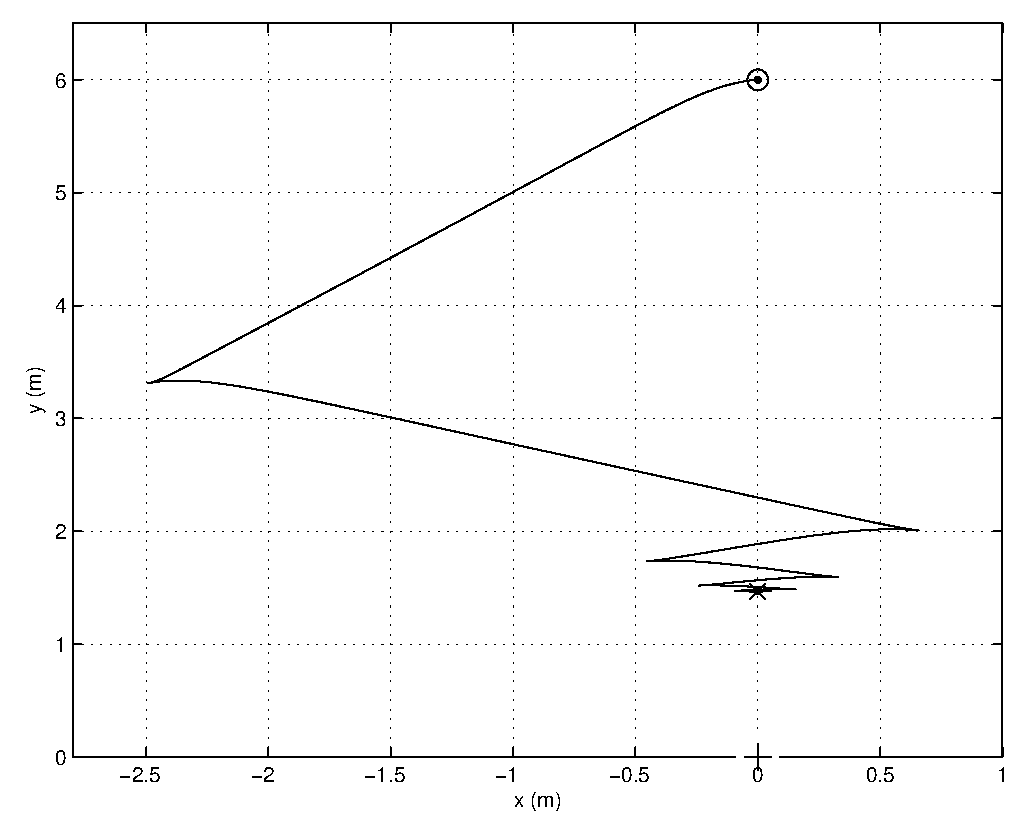
\includegraphics[width=\linewidth]{Figures/traj_01.eps}
    \caption{Trajectory in the XY-plane.}
    \label{fig:traj_01}
\end{figure}
\begin{figure}[htbp]
	\centering
    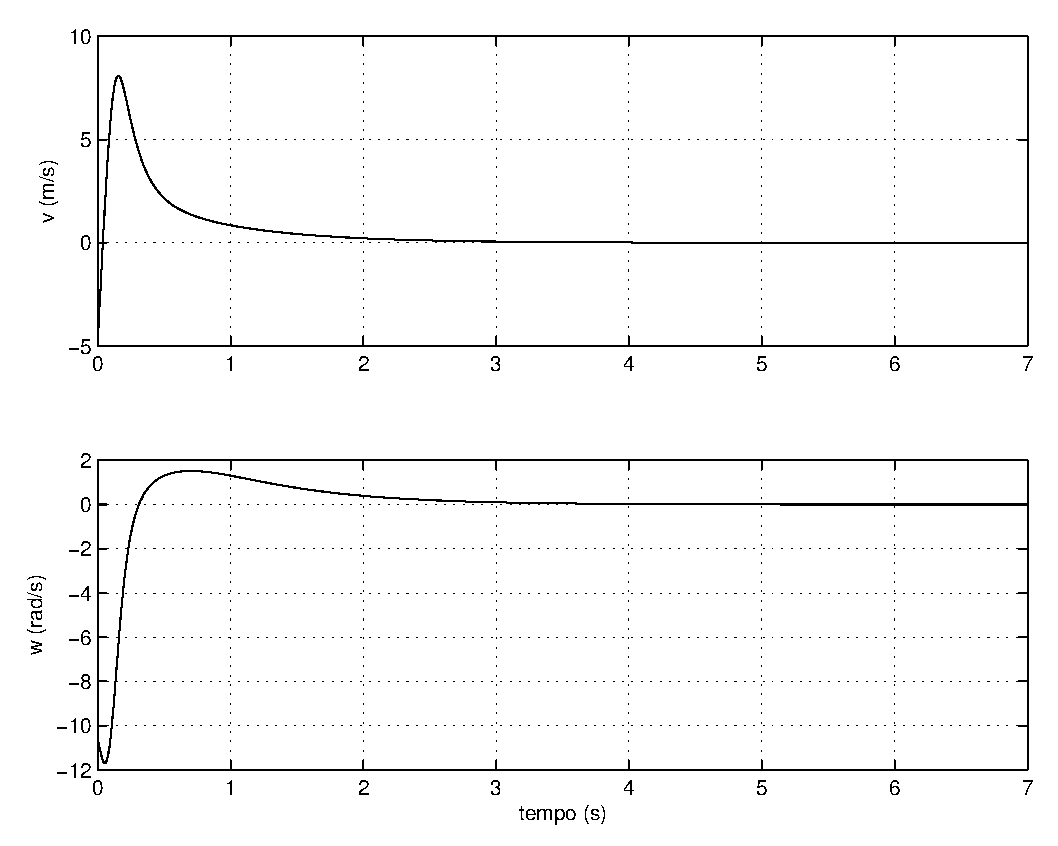
\includegraphics[width=\linewidth]{Figures/control_01.eps}
    \caption{Control inputs.}
    \label{fig:control_01}
\end{figure}
\begin{figure}[htbp]
	\centering
    	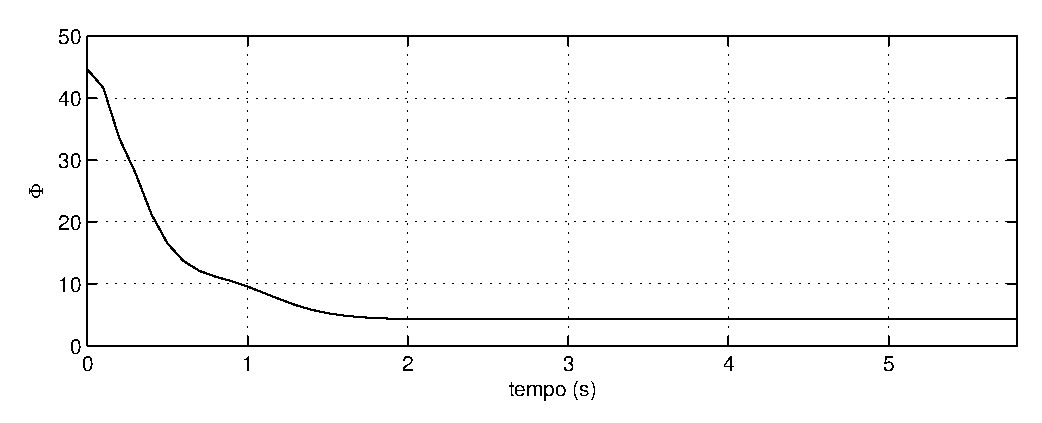
\includegraphics[width=\linewidth]{Figures/cost_01.eps}
    	\caption{Cost Function.}
    	\label{fig:cost_01}
\end{figure}

Fig.~\ref{fig:traj_01} shows the trajectory of the robot in the XY-plane, Fig.~\ref{fig:control_01} shows the control inputs bounded by the imposed constraints and Fig.~\ref{fig:cost_01} is the cost function. It is straightforward to note that there is a large steady-state error in one of the position variables ($y$-state, in this case). Notice also that the robot has already stopped since both control inputs converge to zero. The final configuration is ${\bf x}_f=[0~~1.47~~0]^T$. 
\fimex
\end{ex}

This issue can be  explained by the fact that, examining the kinematic model of the Eq.~\req{eqn:model}, both states, $x$ and $y$, depends on the same control variable, the linear velocity $v$. Thus, when the optimization algorithm minimizes $v$ and $x$, it can no more minimizes $y$. Notice that the cost function in Fig.~\ref{fig:cost_01} obbeys a monotonic decreasing behavior and its final value is not zero. In~\cite{kuhne05} is shown that, by increasing considerably the prediction horizon, this problem can be strongly reduced. However, long prediction horizons are in general undesirable since the computational effort is directly related to it.

This offset problem was also identified in~\cite{essen01}, and trying to eliminate this steady-state offset, some modification in the cost functions were proposed in order to increase the state penalty over the horizon, thus forcing the states to converge to an acceptable solution. Hence, in this work the idea of exponentially increasing wheighting factors in the state variable is introduced. Furthermore, a terminal state cost is added to the cost function to be minimized.

\begin{ex}\label{ex2}
Then, including the idea developed in~\cite{essen01} to the cost function, the following cost function can be formulated:
\begin{multline}\label{eqn:essen_cost}
	\Phi(k) = \sum_{j=1}^{N-1}{\bf x}^T(k+j|k){\bf Q}(j){\bf x}(k+j|k) + \\ + \sum_{j=0}^{N-1}{\bf u}^T(k+j|k){\bf R}{\bf u}(k+j|k) + \Omega({\bf x}(k+N|k)),
\end{multline}
where $\Omega({\bf x}(k+N|k)) = {\bf x}^T(k+N|k){\bf P}{\bf x}(k+N|k)$ and ${\bf Q}(j) = 2^{j-1}{\bf Q}$.
Using the same tunning parameters and the same initial condition as in Example~\ref{ex1}, and with a terminal state wheigthing of ${\bf P}=50{\bf Q}(N)$, he have the simulation results shown in Fig's~\ref{fig:traj_02}-\ref{fig:cost_02}.
\begin{figure}[htbp]
	\centering
	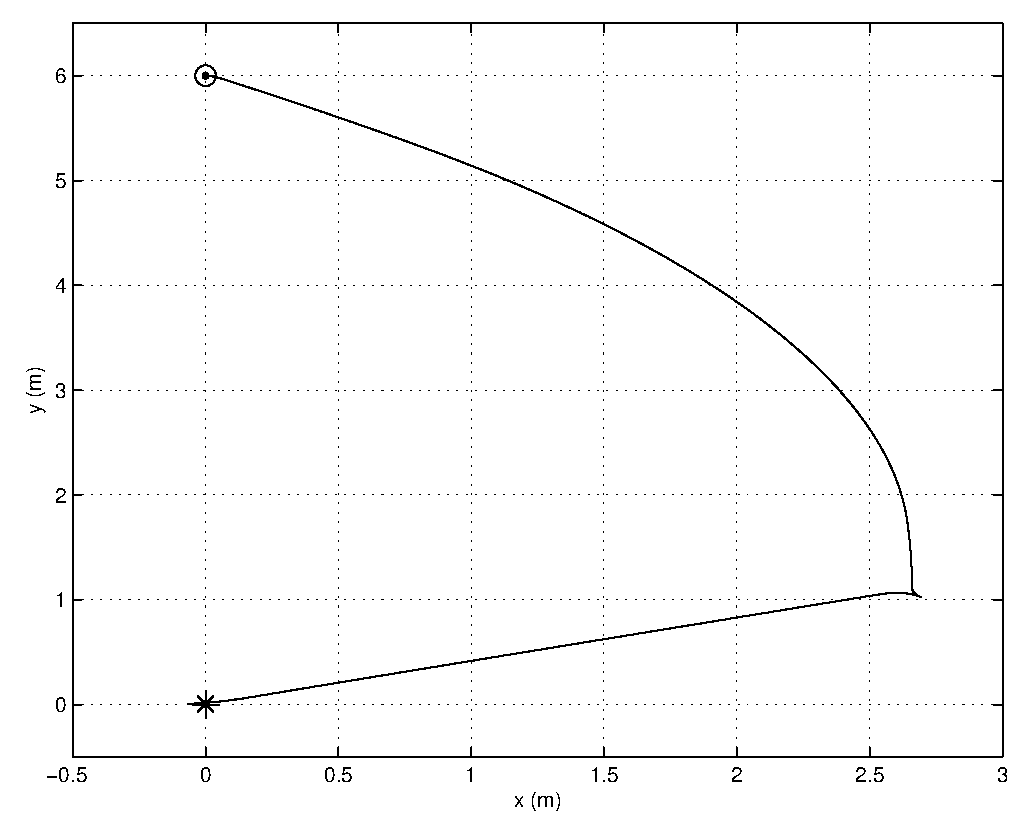
\includegraphics[width=\linewidth]{Figures/traj_02.eps}
   	\caption{Trajectory in the $XY$ plane.}
   	\label{fig:traj_02}
\end{figure}
\begin{figure}[htbp]
	\centering
   	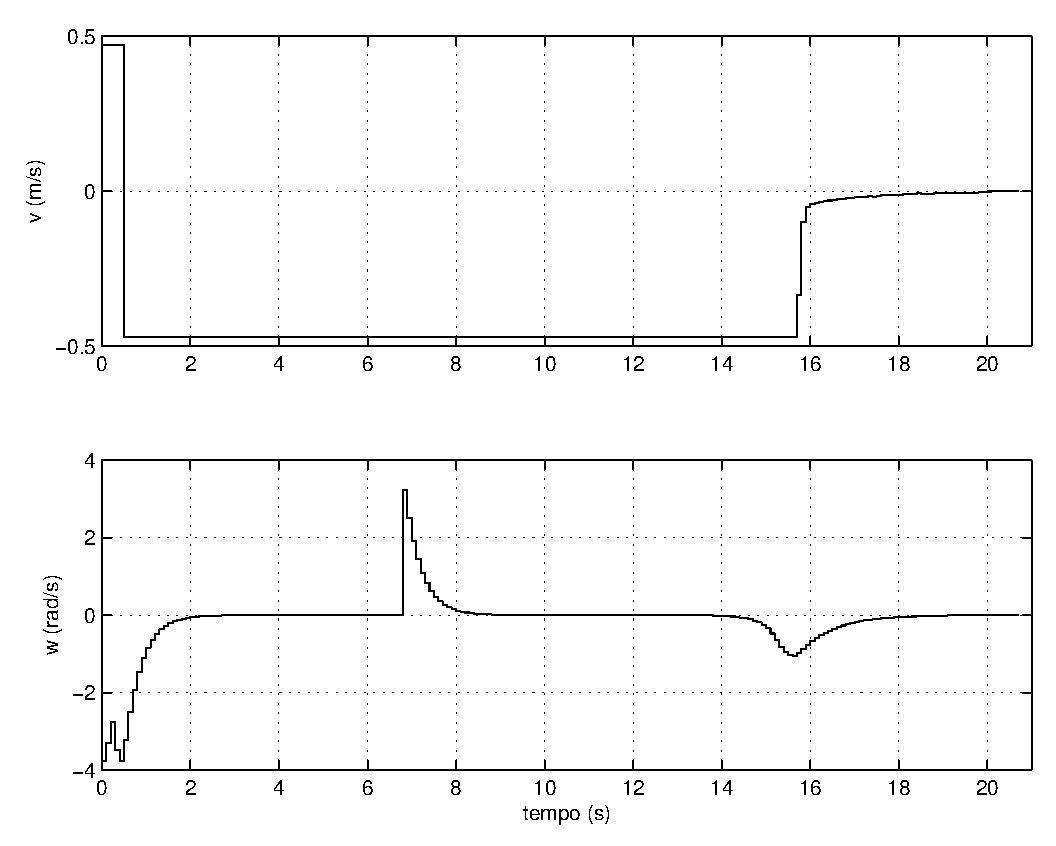
\includegraphics[width=\linewidth]{Figures/control_02.eps}
   	\caption{Control inputs.}
   	\label{fig:control_02}
\end{figure}
\begin{figure}[htbp]
	\centering
    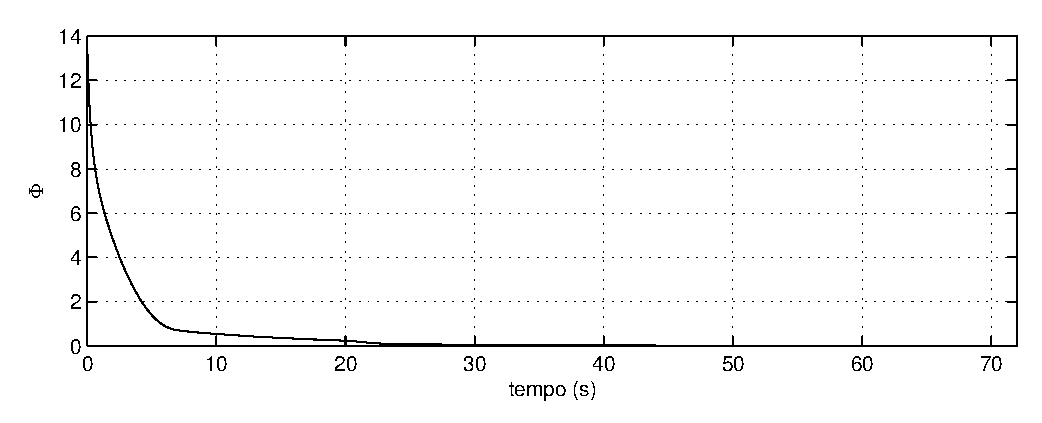
\includegraphics[width=\linewidth]{Figures/cost_02.eps}
    \caption{Cost function.}
    \label{fig:cost_02}
\end{figure}

Then, it can be clearly seen in Fig.~\ref{fig:traj_02} that the large steady-state offset in $y$-state has disappeared. Also, notice in Fig.~\ref{fig:control_02} that the convergence rate, in comparison to the Example~\ref{ex1}, is higher. In the first example the stabilization time is about 40 seconds, while now this is 21 seconds. The control signals respect the imposed constraints. Fig.~\ref{fig:cost_02} shows the monotonicaly decreasing behavior of the cost function.

However, the coupling between the states $x$ and $y$ continue to exists. The final $y$-state still presents a persistent offset. The final configuration is ${\bf x}_f=[0~~0.006~~0]^T$. 
\fimex
\end{ex}

Then, it is easy to realize that the solution to this problem could be to find some coordinate transformation such that the position states $x$ and $y$ are decoupled from the same control input $v$. Thus, based in the work of \cite{lages98b}, now we will introduce this idea, using the following state transformation into polar coordinates:
\begin{equation*}
	e = \sqrt{x^2+y^2}, \qquad 
	\phi = \atan(y,x), \qquad
	\alpha = \theta - \phi,
\end{equation*}
and the following Lyapunov function:
\begin{equation}\label{eqn:lyapunov}
	V = \frac{1}{2}\left(\lambda e^2 + h\phi^2 + \alpha^2\right),
\end{equation}
where $\lambda$ and $h$ are positive constants. Eq.~\req{eqn:lyapunov} can be rewritten in a quadratic form as:
\begin{equation*}
	V = {\bf x}_p^T{\bf Q}_p{\bf x}_p, \qquad
	{\bf x}_p=\begin{bmatrix} e \\ \phi \\ \alpha \end{bmatrix}, \qquad
	{\bf Q}_p = \begin{bmatrix}
		\frac{1}{2}\lambda & 0 & 0 \\
		0 & \frac{1}{2}h & 0 \\
		0 & 0 & \frac{1}{2}
	\end{bmatrix}
\end{equation*}

Considering also a control penalty term, the following cost function can therefore be formulated:
\begin{multline}\label{eqn:polar_cost}
	\Phi_p(k) = \sum_{j=1}^{N}{\bf x}_p^T(k+j|k){\bf Q}_p{\bf x}_p(k+j|k) + \\ + {\bf u}^T(k+j-1|k){\bf R}{\bf u}(k+j-1|k)
\end{multline}

\begin{ex}\label{ex3}
In this example the NMPC will be solved with the cost function in polar coordinates of Eq.~\req{eqn:polar_cost}. Then, with the same tunning parameters and initial condition used in the others two examples, he have the following results showed in Fig's~\ref{fig:traj_03}-\ref{fig:cost_03} below.
\begin{figure}[H]
	\centering
	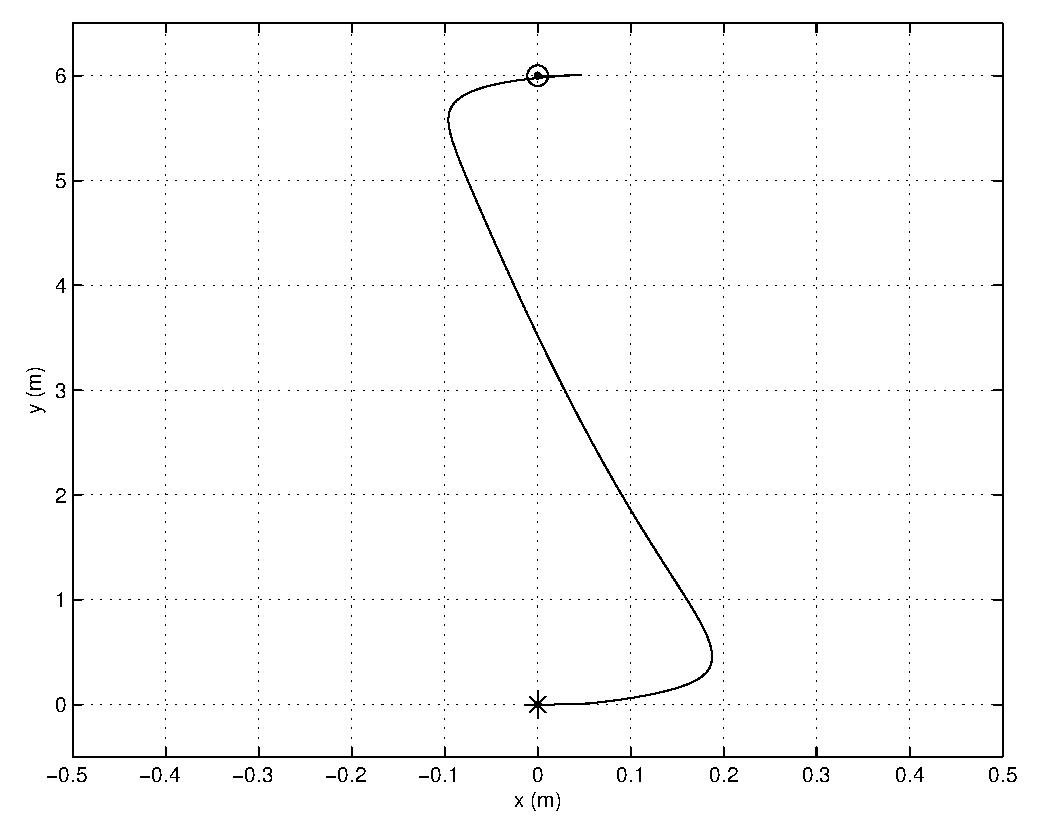
\includegraphics[width=\linewidth]{Figures/traj_03.eps}
   	\caption{Trajectory in the $XY$ plane.}
   	\label{fig:traj_03}
\end{figure}
\begin{figure}[H]
	\centering
   	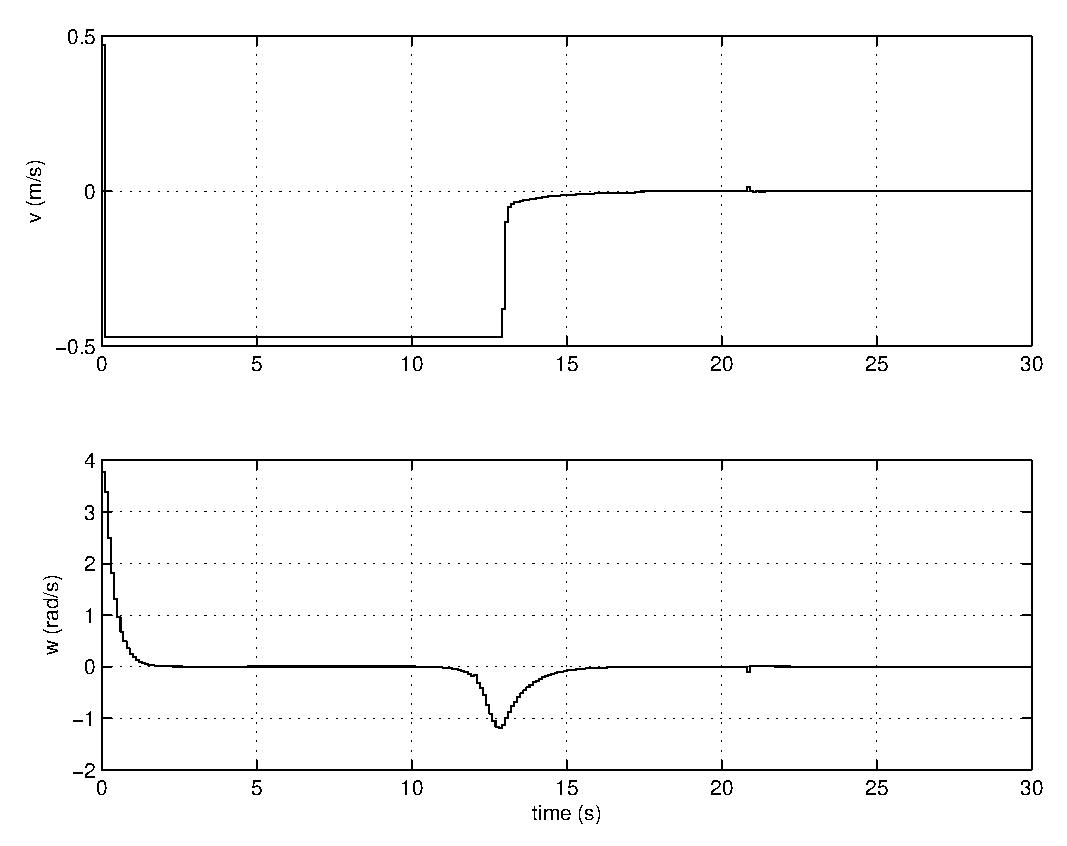
\includegraphics[width=\linewidth]{Figures/control_03.eps}
   	\caption{Control inputs.}
   	\label{fig:control_03}
\end{figure}
\begin{figure}[H]
	\centering
    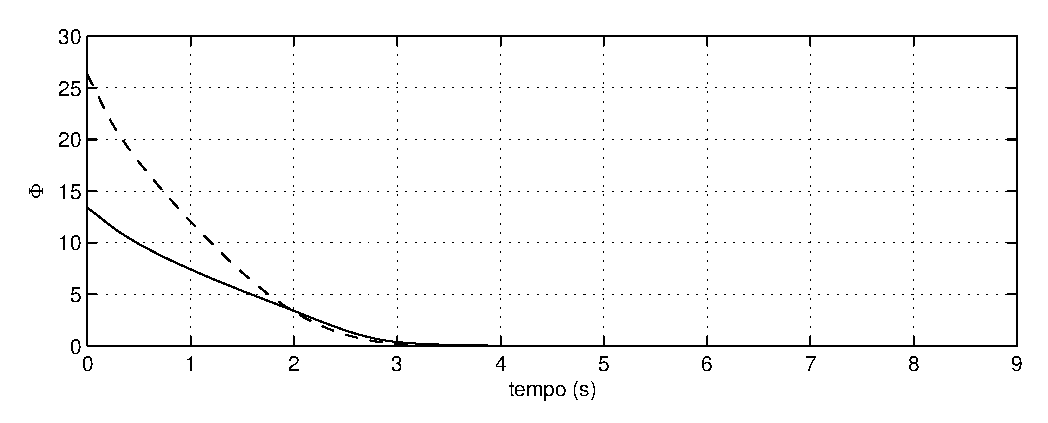
\includegraphics[width=\linewidth]{Figures/cost_03.eps}
    \caption{Cost function.}
    \label{fig:cost_03}
\end{figure}

Then, comparing the results above with the results obtained in Example~\ref{ex2}, significative performance improvements with respect to both state and control trajectories can be noted. The robot needs about 16 seconds to achieve its objective, against 40 seconds and 21 seconds of the Examples~\ref{ex1} and \ref{ex2}, respectively. It is easy to see in Fig.~\ref{fig:traj_03} that the $x$-state developes a maximum amplitude of about $0.3~m$, while for the Example~\ref{ex2} the $x$-state needs almost $3~m$ to maneuver towards the origin (Fig.~\ref{fig:traj_02}). In Fig.~\ref{fig:control_03} the control inputs are smoother than the presented in Fig.~\ref{fig:control_02}. The monotonicaly decreasing behavior of the cost function is shown in Fig.~\ref{fig:cost_03}.

Thus, with the transformation of the cost function in polar coordinates, it has been possible the decoupling between the position states $x$ and $y$. Now the final configuration is ${\bf x}_f=[0~~0~~0]^T$. Furthermore, it has been possible to improve the overall performance without the inclusion of another terms in the cost function or a longer prediction horizon. 
\fimex
\end{ex}


%%%%%%%%%%%%%%%%%%%%%%%%%%%%%%%%%%%%%%%%%%%%%%%%%%%%%%%%%%%
\section{The Computational Effort}\label{sec:comp}
The use of MPC for real-time control of systems with fast dynamics such as a WMR has been hindered for some time due to its numerical intensive nature~\cite{cannon00}. However, with the development of increasingly faster processors the use of MPC in demanding applications becomes possible. 

As measurement criterion, the number of floating point operations per second (flops) was used.

An Athlon XP 2600+ gives a peak performance between 576 and 1100 Mflops using double precision computations accordingly to~\cite{aburto92}, a de-facto standard for floating point performance measurement. 

The data presented in Table~\ref{tab:comp} below refers to the mean value of floating point operations per sampling time along the developed trajectory for the three examples in Section~\ref{sec:results} for a sampling period of $T=100~ms$. Example~\ref{ex1} is the NMPC with the original cost function, Eq.~\req{eqn:cost}; Example~\ref{ex2} is the NMPC with the cost function of~\cite{essen01}, Eq.~\req{eqn:essen_cost}; and Example~\ref{ex3} is the NMPC with the proposed cost function, eq.~\req{eqn:polar_cost}, in polar coordinates.

\begin{table}[H]
	\label{tab:comp}
	\renewcommand{\arraystretch}{1.3}
	\centering
	\caption{The Computational Effort.}
	\begin{tabular}{c|ccc}
	\hline
			& \multicolumn{3}{c}{Mflops} \\
	Horizon   & Example~\ref{ex1} & Example~\ref{ex2} & Example~\ref{ex3} \\
	\hline\hline
	5	& 6.41 & 14   & 8.17 \\
	10	& 114  & 384  & 128  \\
	12	& 246  & 926  & 434  \\
	15 	& 626  & 6077 & 1392 \\
	\hline
	\end{tabular}
\end{table}

Hence, the data in Table~\ref{tab:comp} provides enough evidence that a standard of-the-shelf computer is able to run a MPC-based controller for a WMR. Note that for $N=5$ all of the examples are feasible in real-time. However, results presented in Example~\ref{ex1} show the existence of steady-state offset and the results in Example~\ref{ex2} show poor performance. Thus, among all of them, the approach that performs the best results with respect to state and control trajectories and computational effort is the one proposed in Example~\ref{ex3}, the NMCP with cost function in polar coordinates.


%%%%%%%%%%%%%%%%%%%%%%%%%%%%%%%%%%%%%%%%%%%
\section{Conclusion}\label{sec:conclusions}

This paper presented an application of model predictive control to the problem of point stabilization of a nonholonomic wheeled mobile robot. A steady-state offset in one of the position variable has been identified and a transformation of the configuration variables into polar coordinates has been successfully solved the problem. Through some examples, it was shown an important advantage of MPC: to handle constraints ina straightforward way durng the computation of the control law. The obtained control signals were such that the constraints imposed on the control variables were respected. 

As shown above, the choice of MPC for the application given here is well justified by some advantages: the existence of a performance criterion which is minimized, thus the control law is optimal with respect to this minimization; the straightforward way in which state/input constraints can be handled; the MPC implicitly generates a control law that deal with Brockett conditions.

Furthermore, considerations regarding the computational effort of the MPC were developed with the purpose of speculating the viability of the proposed technique in a real implementation. It has been shown that with the proposed technique the NMPC can be applied to a WMR in real-time.

\section*{Acknowledgments}

The authors gratefully acknowledge the financial support from CAPES.

% Equaliza as colunas da �ltima p�gina:
\IEEEtriggeratref{5}

\bibliographystyle{IEEEtran}
\bibliography{icma05}

\end{document}
